\documentclass[12pt]{exam}
\usepackage{booktabs}
\usepackage[hmargin=1.5cm, top=1.5cm, bottom=2cm]{geometry}
\usepackage[T1]{fontenc}
\usepackage[utf8]{inputenc}
\usepackage[portuguese]{babel}
\usepackage{graphicx}
\usepackage{tikz}
\usepackage{titling}
\usepackage{indentfirst}
\usepackage{subcaption}
\usepackage{enumitem}
\usepackage{pifont}
\usepackage{siunitx}
\usepackage{adjustbox}
\usepackage{hyperref}
\usepackage{interval}
\usepackage{microtype}

\graphicspath{ {./output} }
\setlength{\droptitle}{-5em}
\renewcommand\_{\textunderscore\linebreak[1]}
\cfoot{\normalsize\thepage}

\author{Grupo: al020\\Alunos: Duarte Almeida (ist195565) e Gustavo Aguiar (ist195587)}
\title{Numbrix IA P3 2021/2022}
\date{}\date{}

\begin{document}
    \maketitle
    \begin{tikzpicture}[overlay, remember picture]
        \node[xshift=3.5cm,yshift=-2cm] at (current page.north west) {
\includegraphics[scale = 0.35]{logo_ist.jpeg}};
    \end{tikzpicture}
    \vspace{-6em}
    \section{Descrição do Problema e da Solução}
        \indent No âmbito da UC de Inteligência Artificial, foi-nos proposto solucionar o problema \textit{Numbrix}.
        Neste existe uma grelha \textbf{$N\times N$}, onde cada célula pode conter um número positivo inteiro.
        O objetivo é preencher a grelha com uma sequência de números adjacentes horizontal ou verticalmente, com base numa instância inicialmente
        dada que já contém posições fixas de números em células.

        \indent Como auxílio de resolução ao problema, foram usados os vários algoritmos de procura informada e não informada disponibilizados no ficheiro \textit{search.py} — mais concretamente, os seguintes: \textit{breadth\_first\_tree\_search}, \textit{depth\_first\_tree\_search}, \textit{astar\_search}, \textit{greedy\_search}.

        \indent A \textbf{solução} utilizada para a resolução do problema foi uma que cria ilhas ordenadas de números no tabuleiro (seja o conjunto dessas ilhas \textbf{I}). O algoritmo implementado tenta sucessivamente ligar o maior número da menor ilha ($I_{0}$) ao menor número da segunda menor ($I_{1}$), até que convirja em 1 só. Define-se uma ilha de números, $I_{j}$, como uma sequência de números adjacentes que são células vizinhas no tabuleiro, como abaixo exemplificado.
        \vspace{-2.5mm}
        \begin{table}[ht!]\centering\footnotesize
            \begin{subtable}{0.2\textwidth}
                \centering
                \begin{tabular}{ccc}
                    2 & 3 & 0 \\
                    1 & 0 & 0 \\
                    0 & 0 & 0
                \end{tabular}
                \caption{\textbf{I} = $\{\{1, 2, 3\}\}$}
            \end{subtable}
            \hfill
            \begin{subtable}{0.2\textwidth}
                \centering
                \begin{tabular}{ccc}
                    2 & 0 & 4 \\
                    1 & 0 & 5 \\
                    0 & 0 & 0
                \end{tabular}
                \caption{\textbf{I} = $\{\{1, 2\}, \{4, 5\}\}$}
            \end{subtable}
            \hfill
            \begin{subtable}{0.2\textwidth}
                \centering
                \begin{tabular}{ccc}
                    5 & 4 & 1 \\
                    0 & 3 & 0 \\
                    0 & 0 & 0
                \end{tabular}
                \caption{\textbf{I} = $\{\{1\}, \{3, 4, 5\}\}$}
            \end{subtable}
        \end{table}

        \vspace{-3.5mm}
        \indent As \textbf{ações} a serem executadas a partir de um dado estado dependem de \#\textbf{I} (seja $x = min(I_{0})$ e $y = max(I_{0})$):\\
        \vspace{-6.5mm}
        \begin{itemize}[label=\ding{212}]
          \setlength\itemsep{-0.2em}
            \item Se $\#\textbf{I} > 1$, para cada célula adjacente livre\footnote{Uma célula diz-se livre se não está preenchida por nenhum número no tabuleiro.} de $y$ meter $z = y + 1$.
            \item Se $\#\textbf{I} = 1$, no caso de $x \neq 1$ meter $z_{1} = x - 1$ para cada célula adjacente livre da posição de $x$ e, analogamente, no caso de $y \neq N^2$ meter $z_{2} = y + 1$ para cada célula adjacente livre da posição de $y$.
        \end{itemize}
        \vspace{-3mm}

        \indent O \textbf{resultado} das ações consiste em copiar as estruturas do tabuleiro e auxiliares, definir a nova posição dada pelas ações e realizar a possível convergência de ilhas.

        \indent A \textbf{heurística} implementada tem em conta os seguintes aspetos (seja ainda $x = max(I_{0})$, $y = min(I_{1})$ e $g_{min} = min(I_{0})$ e $g_{max} = max(I_{N})$, assumindo para $y$ que \textbf{I} contém $N > 1$ ilhas):
        \vspace{-2mm}
        \begin{itemize}[label=\ding{212}]
          \setlength\itemsep{-0.2em}
            \item Se não existem $g_{min} - 1$ posições livre desde a posição de $g_{min}$ ou $N^2 - g_{max}$ desde a posição de $g_{max}$, devolve $\infty$.
            \item Se $\#\textbf{I} > 1$, se $Manhattan(pos_{x}, pos_{y}) > x - y$, ou se a posição de $y$ não é atingível por $x$, ou se a ação cria \textit{dead spaces}\footnote{Um \textit{dead space} no tabuleiro é um sub-conjunto de posições livres que torna impossível qualquer tipo de preenchimento coerente com as restrições do problema.} no tabuleiro, devolve $\infty$.
            \item Para cada célula livre no tabuleiro, contar o seu número de células livres adjacentes e elevar esse número a $1.4$. No fim, devolver a soma desta contagem de todas as células livres.
        \end{itemize}


    \section{Implementação e Análise dos Resultados}~
        \indent Dados os testes de \textit{input/output} fornecidos pelo corpo docente, obtiveram-se os seguintes resultados aplicando o algoritmo implementado:\\

        \begin{adjustbox}{width={\textwidth}, totalheight={\textheight}, keepaspectratio}
        \begin{tabular}{l cccc cccc cccc}
        \toprule
         & \multicolumn{4}{c}{Tempo de Execução (s)} & \multicolumn{4}{c}{Nós Gerados} & \multicolumn{4}{c}{Nós Expandidos}\\
        \cmidrule(lr){2-5} \cmidrule(lr){6-9} \cmidrule(lr){10-13}
        Input           & BFS  & DFS  & A* & GS       & BFS  & DFS  & A* & GS        & BFS  & DFS  & A* & GS \\
        \midrule
        1               & 0.0004 & 0.0003  & 0.0008    & 0.0008            & 10    & 7 & 7    & 7       & 10   & 5   & 5      &5  \\
        2               & 0.4837 & 0.1165  & 0.3179    & 0.3314            & 7280  & 1218 & 779  & 834       & 7270   & 1199   & 493    &516  \\
        3               & 0.0852 & 0.0360  & 0.0158    & 0.0147            & 2186  & 991 & 59   & 54       & 2184   & 980   & 34     &32  \\
        4               & 0.3192 & 0.1758  & 0.0630    & 0.0611            & 4473  & 2898 & 230  & 230       & 4473   & 2887   & 118    &118  \\
        5               & 0.2385 & 0.0176  & 0.1479    & 0.0454            & 5760  & 430 & 516  & 188       & 5760   & 420   & 302    &107  \\
        6               & 0.1693 & 0.0633  & 0.1000    & 0.0998            & 2857  & 1092 & 199  & 199       & 2857   & 1076   & 111    &112  \\
        7             & 106.1534 & 39.4617  & 0.4971    & 0.3778         & 1343928  & 714831 & 928  & 744       & 1343928   & 714802   & 437    &365  \\
        8               & 0.5891 & 0.2635  & 0.4280    & 0.4117            & 4611  & 2653 & 599  & 588       & 4584   & 2634   & 386    &380  \\
        9               & 0.6193 & 0.2668  & 0.4232    & 0.4134            & 4611  & 2653 & 599  & 588       & 4584   & 2634   & 386    &380  \\
        10              & 0.1804 & 0.0536  & 0.2072    & 0.1835            & 2303  & 957 & 338  & 312       & 2303   & 943   & 232    &215  \\
        \bottomrule
        \end{tabular}
        \end{adjustbox} \\

        \indent Primeiramente, o uso da heurística foi um elemento nitidamente diferenciador. Porém, dada a impossibilidade de apurar qual dos algoritmos a usar a heurística (\textit{A-Star Search} ou \textit{Greedy Search}) era o mais eficiente, criou-se uma \href{https://github.com/ImGugz/IA2122/blob/main/src/generator.py}{ferramenta em \textit{Python}} que gerava ficheiros \textit{input/output} que nos permitissem ver a fundo como otimizar a heurística. Para o efeito, geraram-se 6 instâncias de tabuleiros $10 \times 10$ e utilizaram-se ambos os algoritmos com a mesma heurística, com incrementos de $0.2$ no expoente da heurística, $j$, tal que $j \in \interval{1}{2}.$
        \vspace{-4.5mm}
        \begin{figure}[ht!]
        \centering
        \subfloat[\centering \textit{A-Star Search}]{{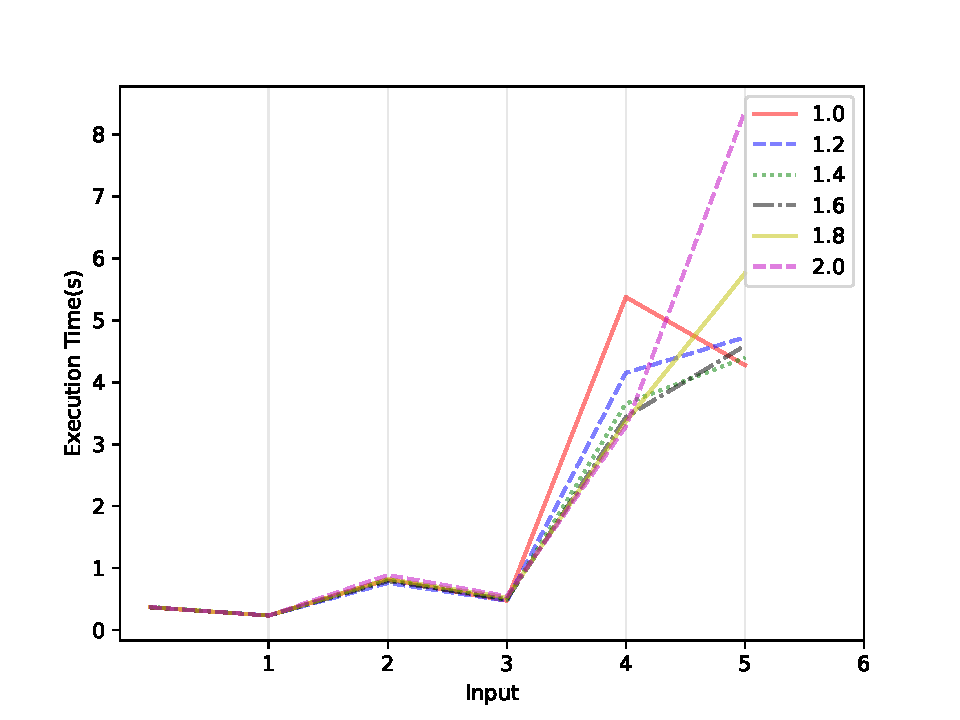
\includegraphics[width=8.5cm]{a-star_h_plot.pdf} }}%
        \qquad
        \subfloat[\centering \textit{Greedy Search}]{{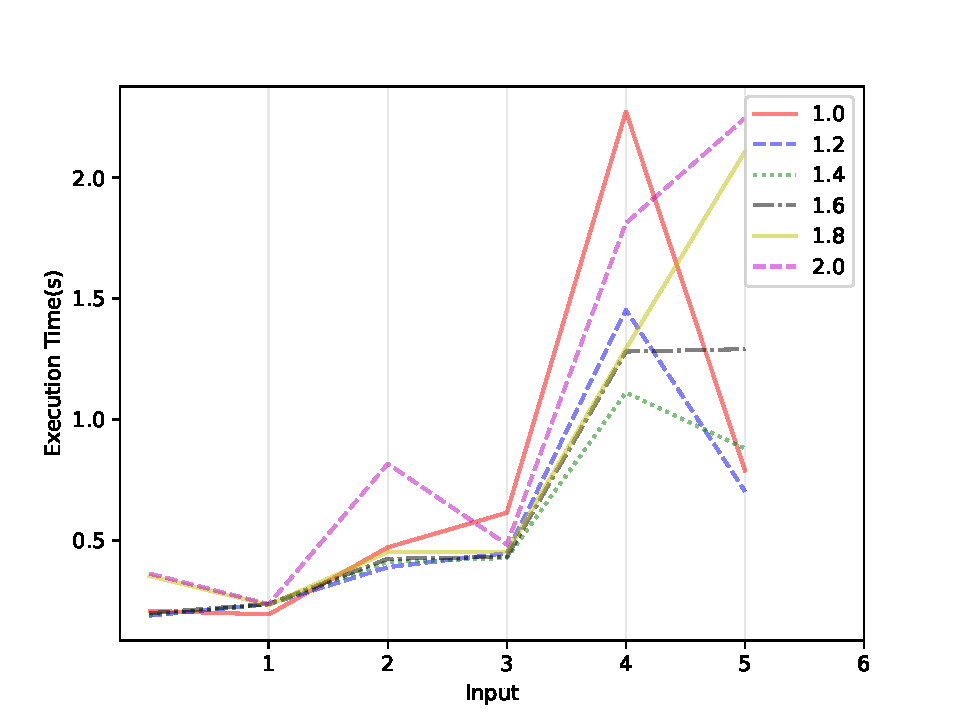
\includegraphics[width=8.5cm]{greedy_h_plot.pdf} }}%
        \caption{Comparação do expoente da heurística entre \textit{A-Star Search} e \textit{Greedy Search}}%
        \label{fig:example}%
        \end{figure}

        \indent Verificou-se que para os mesmos testes o algoritmo \textit{Greedy Search} conseguiu uma redução significativa de tempo de execução. Para além dessa análise experimental feita, destacou-se o facto de o expoente $1.4$ ser em média o que mais reduzia o tempo de execução. Por fim, considerando todos os fatores supramencionados, decidiu-se optar pela implementação com \textbf{procura informada que usa o algoritmo \textit{Greedy Search} e expoente 1.4 na heurística}.

\end{document}
